\documentclass[12pt, a4paper]{extarticle}

\usepackage[left=1.25in,right=1in,top=1in,bottom=1in]{geometry}
\usepackage {fancybox}
\usepackage{graphicx}
\usepackage{hyperref}
\usepackage{ragged2e}
\usepackage{times}

\hypersetup{
    colorlinks=true,
    linkcolor=black,     
    urlcolor=cyan,
}

\begin{document}

    \pagenumbering{gobble}
    
    \begin{titlepage}
% 		\thispagestyle{empty}
		\thisfancypage{\setlength{\fboxsep}{1pt}\doublebox}{}		
		\begin{center}
    		\includegraphics[scale=0.45]{images/head.jpeg}    		
    		
    		\vspace{0.5in}
			Research report for the Final Year Project
			
			\vspace{0.125in}
			{\Large \textbf{`` Epidemic Simulation ''}}
			
			\vspace{1in}
			Under the guidance of
			
			\vspace{0.125in}
			\textbf{Dr. H C Vijayalakshmi}
		\end{center}			
		\vspace{0.5in}
		
		\hspace{0.25in}Team Number: 26
		
		\hspace{0.25in}Team Members:	
		\vspace{0.125in}
        \begin{table}[h!]
            \begin{center}
                \begin{tabular}{|c|c|c|c|} \hline
                	\textbf{USN} & \textbf{Name} & \textbf{Section} & \textbf{Roll No.} \\ \hline
    	            01JST17CS052 & Eeshaan Achar & C & 16\\ \hline
	                01JST17CS024 & Anuj Yadav & C & 8\\ \hline
            	    01JST17CS142 & Saurav Kumar & C & 40\\ \hline
        	        01JST17CS080 & Manjunath Badakar & C & 22\\ \hline
                \end{tabular}
            \end{center}
		\end{table}
		
        \vspace{1.5in}
		\hspace{0.25in}Signature of Guide \hspace{2.3in} Signature of HOD
		
		\hspace{0.1in}(Dr. H C Vijayalakshmi) \hspace{1.9in} (Dr. M P Pushpalatha)		
		
		\vspace{0.25in}
		\begin{center}       
            \textbf{Department of Computer Science and Engineering\\2020-21}	
		\end{center}
	\end{titlepage}
    
    \newpage
    % \thispagestyle{empty}
    \begin{titlepage}
        \thisfancypage{
            \setlength{\fboxsep}{1pt}
            \doublebox
        }{}
        \begin{center}
            \includegraphics[width=150mm]{images/head.jpeg}
            \textbf{\large{\underline{CERTIFICATE}}}
            \vspace{1in}
            
            \justifying
                This is to certify that the final year project presentation titled \textbf{``Epidemic Simulation"} is presented by \textbf{Eeshaan Achar, Anuj Yadav, Saurav Kumar} and \textbf{Manhunath Badakar} for the partial fulfillment of the award of the degree of Bachelor of Engineering in Computer Science and Engineering, at JSS Science \& Technology University, Mysuru during the year 2020-21. It is certified that all corrections / suggestions suggested during the presentation have been incorporated in the report. The report has been approved as it satisfies the academic requirements with respect to the final year project presentation prescribed for the Bachelor of Engineering degree.
            
            \vspace{2in}
            \flushleft\hspace{1.75cm}\textbf{Signature of Guide} \hspace{5cm}\textbf{Signature of HOD}
            \flushleft\hspace{1.25cm}\textbf{(Dr. H C Vijayalakshmi)} \hspace{4cm}\textbf{(Dr. M. P. Pushpalatha)}
            \vspace{0.5in}
            \flushleft\hspace{2cm}\textbf{Panel Members} \hspace{6cm}\textbf{Signature}
            \vspace{6mm}
            \flushleft \hspace{1cm}1. .........................................
            \hspace{4.25cm}..................................
            \newline
            \flushleft \hspace{1cm}2. .........................................
            \hspace{4.25cm}..................................
            \newline
            \vspace{5mm}
            \flushleft\hspace{1cm}\textbf{Date:} \hspace{8cm}\textbf{Place:}
        \end{center}
    \end{titlepage}
    
    \newpage
    % \thispagestyle{empty}
    \section*{Declaration}
        \paragraph{} We, the undersigned, solemnly declare that the report of the research work entitled ``Epidemic Simulation", is based on our own work carried out during the course of our study at JSS Science and Technology University Mysore, under the supervision of Dr. H C Vijayalakshmi. We assert that the statements made and conclusions drawn are an outcome of the research work. We further declare that to the best of our knowledge and belief that the project report.
        
        \vspace{5in}
        \hspace*{4in} Eeshaan Achar
        
        \vspace{0.75in}
        \hspace*{4in} Anuj Yadav
        
        \vspace{0.75in}
        \hspace*{4in} Saurav Kumar
        
        \vspace{0.75in}
        \hspace*{4in} Manjunath Badakar

	\newpage
    % \thispagestyle{empty}
    \section*{Abstract}
        \paragraph{} This document is the concluding report of our research project entitled ``Epidemic Simulation", and is prepared as per the guidelines issued by the Department of Computer Science and Engineering, JSS Science and Technology University Mysore. In this document, we have covered every important aspect of the research to the best possible extent, and we hope that the anyone reading this would not only understand the research but would also find it worthy of his / her time.
    
    \newpage
    % \thispagestyle{empty}
    \section*{Acknowledgement}
        \paragraph{} This research has been made possible by the kind support of many individuals such as our friends and families, and organizations such as our university. We wish to extend our sincere gratitude to all of them. We would also like to express gratitude to our mentor Dr. H C Vijayalakshmi, as without her guidance in the past as well as in the coming days, this project would not have been feasible. Lastly, we would like to thank our fellow teammates for their time and efforts, without which this project would not have seen the light of the day.

    \newpage
% 	\thispagestyle{empty}
	\tableofcontents
	
	\newpage
	\pagenumbering{arabic}
    \section{Introduction}
        \subsection{Problem Statement}
            \paragraph{} An Epidemic is an outbreak of a disease that spreads rapidly and widely. Epidemics such as the Bubonic Plague, Avian flu, H5N1 influenza, H1N1 swine flu, SARS etc. have disturbed human lives for centuries causing massive number of deaths and illnesses among people and animals. As the number of urbanized and mobile population has increased, the possibility of a worldwide pandemic has grown too. The coronavirus pandemic is a testament to the same.
            \paragraph{} Understanding the ways in which diseases propagate has several benefits such as improving healthcare systems, increasing life spans, and reducing the impact of biological warfare. Thus, it is very important for governmental authorities and healthcare agencies to understand how diseases spread and how to limit this spread by selecting the best mitigation and social strategies. Examples of mitigation strategies include vaccination, antiviral treatment, and household prophylaxis. Social distancing strategies include school closure, quarantine, and isolation.
        \subsection{Introduction to Problem Domain}
            \paragraph{} Historically, epidemics have been modelled mathematically to understand their dynamics. These models can vary from a few simple equations to complex systems that need to be simulated on supercomputers. The latest advances in high performance computing and computational network science can help epidemiologists develop large-scale high fidelity models of the epidemic spread. These models can help guide public health officials and policy makers in taking appropriate decisions to prevent and control the epidemics.
        \subsection{Objectives and Scope}
            \paragraph{} Objective is the aim or the final result we wish to achieve by completing a certain process. The scope of a process defines the limitations that we have to face while completing a process. For a successive process, the objectives have to be achieved within the scope.
            \subsubsection{Objectives}
                \begin{itemize}
                    \item Develop a simulation software with an intuitive UI to enable anyone that is interested to simulate the disease spreading and understand its dynamics.
                    \item Simulate the spread of several hypothetical (not necessarily) diseases on several different kinds of population using the said software, and obtain useful information such as the rate of spreading, the rate of recovery of victims, the epidemic duration etc.
                    \item Understand and appreciate the effect of various proposed safety measures such as social distancing, hand washing etc. amidst the prevailing coronavirus pandemic, through the simulation of the same.
                    \item Understand the various social network models available in the literature, along with their working and relevance.
                    \item Appreciate the contributions of various research scholars through their published work, and also propose any improvements if found and feasible.
                \end{itemize}
            \subsubsection{Scope}
                \begin{itemize}
                    \item The simulation will consist of a small sample of population, expected to be around some thousand nodes. This is unlike the real world which consists of over 7 billion humans beings and trillions of other creatures.
                    \item Unlike the real world where the behaviour of people vastly differs from each other and is highly unpredictable, the nodes in our simulated world will have a much more defined behaviour.
                    \item An epidemic will have varied statistics across varying geography. In this simulation however, these statistics will be fed as parameters and will be constant for the entire population.
                    \item There are hundreds of parameters that govern the biological, chemical, and physical dynamics of a disease and its spread through a population. Simulation of all these is impractical, and so we will be going with a small subset of parameters that we believe are the most definitive of an epidemic.
                \end{itemize}
        \subsection{Applications}
            \begin{itemize}
                \item Identifying the critical parameters that contribute the most to the spread of contagions. In other words we can identify what measures can be the most helpful in containing the spread of disease.
                \item Spreading awareness among people and the government about the necessary measures to be taken for handling the spread of the epidemic.
                \item In the event of a future pandemic, we can deduce the various critical parameters according to the situation then, as well as the properties of the new contagion.
                \item Identify the measures that can be taken to minimise economic losses, while still containing the disease.
            \end{itemize}
        \subsection{Existing Solutions}
            \paragraph{} We had taken a look at multiple research papers, articles and videos to look for existing solutions to the said problem statement. However, pretty much all these focus on a particular disease and do not generalise the results to other diseases. Moreover, the simulations are done through a script which is either not available to the public or isn't "well written", making it difficult to execute them and reproduce the results or formulate new discoveries. Nevertheless, these did help us shape this research and a detailed study on all the papers we've referred is in the upcoming sections.
        \subsection{Proposed Solution}
            \paragraph{} In this research, we simulate the spread of a disease on a small population and record the results. Based on the disease, and the various measures taken to limit its spread, we would accordingly tweak the parameters and observe the variations in the result. We would also like to summarize the main technical challenges in this field. For the simulation we have used the basic Susceptible-Infected-Removed model, also called the SIR model. This is a type of compartment model where time is divided into periods and each individual is classified to a particular state in each period. The population is partitioned into three classes: Susceptible (S), Infected (I), and Removed (R). A person who becomes infected moves from class S to class I at a rate which depends on the infectiousness of the virus and the prevalence of infection. Infected individuals who recover from the infection or die from it move to class R.
        \subsection{Research Timeline}
            \paragraph{} Following is the timeline of the research. In January, since we had exams, the work had been paused briefly.
            \begin{figure}[!h]
        		\centering
        		\includegraphics[height=2in, width=6in]{images/GanttChart.png}
        		\caption{Gantt Chart}
            \end{figure}
        
    \newpage
    \section{Literature Survey}
	    \paragraph{} A literature survey is a way to represent the current knowledge, including any substantive findings as well as theoretical and methodological contributions, on a particular topic. Such a survey helps steer the research work to be carried out in a direction that will make it more useful and / or applicable. Therefore, in this section, we go through some of the research papers that aimed to model the pandemics that plagued the 21st century, and thus helped us get a better understanding of our own problem statement.
	    \subsection{SARS: The First Pandemic of the 21st Century}
	       \paragraph{} This paper by James D Cherry \& Paul Krogstad discusses how after an unprecedented global public health effort, the SARS epidemic was controlled within 7 months of its original occurrence. It also examines the unique pediatric aspects of SARS, and reviews the epidemiology with regards to future epidemics. Some of the relevant information derived from this research was that the incubation period of SARS is 2–10 days, with a median of 4–6 days. The attack rate in children is reported to be less than that of adults, but when consideration is given to the large number of nosocomial cases in original data sets, it appears that children have similar rates as adults. The most striking laboratory finding is absolute lymphopenia. This occurred in nearly all pediatric patients. In one study, 57\% percent of children had lymphopenia on presentation, and this frequency rose to 91\% . The mean value was 0.9 ± 0.7 × 9/L. Other frequently abnormal laboratory findings include thrombocytopenia, elevated lactate dehydrogenase, and creatinine phosphokinase. The research concluded that the most important factor in preventing a future epidemic is sound public health policy and the use of standard infection control procedures.
	    \subsection{Strategies for containing an emerging influenza pandemic in Southeast Asia}
	       \paragraph{} In this paper by Neil M. Ferguson and others, published at the time of the H5N1 influenza, the researchers simulated the spread of epidemics on a model of Thailand having 85 million residents. The model included households, schools, and workplaces. Random contacts in the community associated with day-to-day movement and travel were also modeled. They used a metric known as the basic reproduction number, R\textsubscript{0} to analyze the state of the pandemic. R\textsubscript{0} is defined as the average number of secondary cases generated by a typical primary case in an entirely susceptible population. A disease can spread if R\textsubscript{0} \textgreater 1, but if R\textsubscript{0} \textless 1, chains of transmission will inevitably die out. In the simulation, they concluded that for R\textsubscript{0} = 1.5, the epidemic in the modeled population peaks around day 150 and is mostly over by day 200, at which point 33\% of the population has been infected. At R\textsubscript{0} = 1.8, the epidemic peaks around day 100 and infects about 50\% of the population. They further analyzed the effect of social distancing measures, the effect and challenges (such as logistics and supply) of using antiviral prophylaxis. Finally, they concluded that the elimination of a nascent pandemic can best be achieved using a combination of geographically targeted prophylaxis and social distancing measures if the basic R\textsubscript{0} for the virus is below 1.8.
	    \subsection{Mathematical models for devising the optimal Ebola virus disease eradication}
	       \paragraph{} In this research by Shuo Jiang and others, a mathematical model was constructed to devise the optimal Ebola virus disease eradication plan by investigating the numerical spread of Ebola and its eradication pathways. By incorporating hospital isolation and application of medication in the model, and analysing their effect on resisting the spread, it demonstrated the second peak of 10,029 total cases. Using the regional spread of EVD with transmission model analysis, it analysed the numbers of new infections through four important transmission paths including household, community, hospital and unsafe funeral. Based on the result of the model, key paths in different situations were found, and some suggestions were proposed to control regional transmission considering all the Ebola characteristics, economic and time optimization, dynamic factors and local condition constraints etc.
	    \subsection{Homogeneous and network models in Epidemiology}
            \paragraph{} An exact contact network model requires knowledge of every individual in a population and every disease-causing contact between individuals (e.g. sneezing in the case of airborne diseases or sexual contact in the case of sexually transmitted diseases). For even small populations, this is typically unfeasible, and thus the researchers worked with approximate networks. There are several techniques for gathering the information needed to build realistic contact network models. They included tracing all infected individuals and their contacts during an outbreak, surveying individuals in populations and using census, social characteristic or other collected data. The researchers also focused exclusively on static networks, i.e. networks in which contacts are assumed to be fixed during the infectious period of an individual. The permanence of contacts captured by static networks offered a more realistic model of human contact behaviour than that by traditional epidemiological models.
        \subsection{FluTE, a publicly available stochastic influenza Epidemic simulation model}
            \paragraph{} FluTE is an individual-based simulation model of influenza epidemics. In this, researchers described the model's community structure, the natural history of influenza, and simulated interventions. Briefly, all individuals in the model are members of social mixing groups, within which influenza is transmitted by random mixing. The model can simulate several intervention strategies, and these can either change the transmission characteristics of influenza (e.g., vaccination) or change the contact probabilities between individuals (e.g., social distancing). Interventions can occur before the epidemic or in response to an ongoing epidemic.
	        \paragraph{} To help prepare for future influenza seasonal epidemics or pandemics, they developed a new stochastic model of the spread of influenza across a large population. Individuals in this model have realistic social contact networks, and transmission and infections are based on the current state of knowledge of the natural history of influenza. The model has been calibrated so that outcomes are consistent with the 1957/1958 Asian A(H2N2) and 2009 pandemic A(H1N1) influenza viruses. They presented examples of how this model can be used to study the dynamics of influenza epidemics in the United States and simulate how to mitigate or delay them using pharmaceutical interventions and social distancing measures.
        \subsection{Agent-based simulation on avian influenza in Vietnam}
            \paragraph{} In this paper, based on the daily reported number of dead poultry due to avian influenza in northern Vietnam in November of 2005, authors used a mathematical model to estimate the basic reproduction number R\textsubscript{0} of the disease. The significant value of the estimated R\textsubscript{0} explained the explosive outbreak in the poultry population. The authors developed an SIR compartment using a combination of EBM and an ABM to recapture the recorded data of the outbreak of avian influenza and to evaluate the efficiency of existing control measures. Their model assumes a totally homogeneous and well-mixed poultry population where the interaction between infected and susceptible individuals is a random process. The work concluded that the infection process of avian influenza in poultry is not significantly affected by external factors. The results inferred that a comprehensive strategy of culling, bio-security control and large-scale vaccination campaign should be taken promptly to keep the disease under control. Advantages of this approach include evaluation of control and vaccination strategies, as well as combining EBM and ABM. An Assumption was that poultry population was considered to be totally homogeneous and well mixed and this is one of the limitations of this approach.
        \subsection{Cholera Epidemic in Haiti, 2010}
            \paragraph{} In this paper the authors built a compartmental transmission model for the Vibrio Cholera Epidemic in Haiti in 2010 and 2011 and explored potential effects of disease-control strategies. They developed an SIR model with the addition of a water compartment. The water compartment could be contaminated by infected or infectious persons and could in turn infect susceptible persons. The models represented the population of each of Haiti’s ten administrative regions. These populations were combined to form a meta-population model, in which disease could spread both within a given region and between regions reflecting the movement of people between different regions. It was found that Cholera spread between two regions is proportional to the population size of both regions and inversely proportional to the square-distance between regional centroids. Analysis of changes in disease dynamics over time suggests that public health interventions have substantially affected this epidemic. A limited vaccine supply provided late in the epidemic was projected to have a modest effect. One major assumption was that cholera could be transmitted through either close contacts or contaminated water. However, waterborne transmission and consumption of food items contaminated with infective water, which are important ways of cholera transmission, were not considered in this simulation.
        \subsection{Global seasonal occurrence of MERS-CoV infection}
            \paragraph{} This paper aims at investigating the global seasonal occurrence of Middle East Respiratory Syndrome coronavirus (MERS-CoV) outbreaks. The authors obtained the data on the prevalence and occurrence of Middle East Respiratory Syndrome Coronavirus (MERS-CoV) infection from the World Health Organization (WHO) for all the MERS cases reported from the various countries and their allies ministries. The conclusion of this research was that MERS-CoV infection affected 2048 people worldwide; 82\% cases were reported from the Saudi Arabia and 17.96\% cases were reported from other countries worldwide. The maximum number of cases 23.14\% were reported in the month of June. However, low occurrence of infections were seen in the month of January. The health sectors need of awareness programs to mandate implementation of effective control strategies and stringent compliance with better standards of health and hygiene nationwide. The health officials also need to highlight the seasonal occurrence of MERS-CoV suggesting to take the better preventive measures to minimize the disease burden globally.
	    \subsection{The effects of border control and quarantine measures on the\\spread of COVID-19}
            \paragraph{} In this research paper the authors have developed an ``easy-to-use" mathematical framework extending from a meta-population model embedding city-to-city connections to arrange the dynamics of transmission waves caused by imported (people who have been associated with travel history from an epidemic region), secondary, and others from an outbreak source region when control measures are considered. Using the cumulative number of the secondary cases, the authors try to determine the probability of community spread.

            \paragraph{} Using the top 10 visiting cities from Wuhan in China as an example, it is demonstrated that the arrival time and the dynamics of the outbreaks at these cities can be successfully predicted under the reproduction number R\textsubscript{0} = 2.92 and incubation period T = 5.2 days. It is also shown in the study that although control measures can gain extra 32.5 and 44.0 days in arrival time through an intensive border control measure and a shorter time to quarantine under a low R\textsubscript{0} (1.4). The study allows to assess the effects of border control and quarantine measures on the emergence and global spread of COVID-19 in a fully connected world using the dynamics of the secondary cases and demonstrated that after the reporting delay was estimated, the dynamics of the outbreaks at connected cities can be successfully reconstructed using both the imported and the secondary cases. The result implies that all the connected (direct or indirect) countries are having a great risk of outbreak and that if the epidemic growth at the source location is high, even a near full-scale border control without proper quarantine measures, will have only limited effects.
	    \subsection{A Social Network Model of the COVID-19 Pandemic}
	        \paragraph{} This social network model developed by Pei Jun Zhao, Harvard T.H. Chan School of Public Health, provides a conceptual framework to analyze the COVID-19 pandemic on the level of individuals, that can be used to predict the influence of collective social behavior on overall pandemic trajectories. It shows the importance of social distancing, and the message that to contain the epidemic, every member of the public plays a crucial part in breaking the chain of transmission. The social network model of COVID-19 transmission is expandable and extendable. This paper provided a simplified version using population averages for parameters.
        \subsection{Simulation of the COVID-19 epidemic on the social network of Slovenia}
	        \paragraph{} In this paper by Žiga Zaplotnik and others, the researchers developed a virus transmission model on a simplified social network of Slovenia with 2 million nodes organized into home / care center clusters. They found that when the epidemic is uncontrolled, the intrinsic uncertainty mostly originates from the uncertainty in virus transmission, while the randomness of the social network has only minor impact of the final size of the epidemic. The latter is in line with a study, where the social network was constructed based on extensive contact survey data, and which reported only minor impact of reshaping the network structure or removing the variance of connection weights on the final size of the epidemic. On the opposite, in the controlled epidemic with low infected population, the randomness of the social network becomes the major source of forecast uncertainty. They also showed that the uncertainty of the forecast and the associated risk is extremely asymmetric (roughly symmetric on a logarithmic axis) with long exponential tails.

    \newpage
    \section{System Requirements and Analysis}
        \paragraph{} As this is a research-based project, and there are no stakeholders other than us, the researchers, the traditional approach of requirements engineering and SRS documentation isn't applicable here. However, we can try and formalize the goals and objectives of this research in a more systematic way. We can also list out the limited set of requirements for the simulation software.
        \subsection{Requirements Collection}
            \paragraph{} The requirements gathering and negotiation phases were conducted by virtual meetings of the team members and the mentor in the month of November. Further discussions were carried out by the team members over a period of two weeks and clarity was obtained with respect to the research work. It was decided that in order to model the population in our simulation we will be using a SIR model, as the literature survey revealed that most research on this topic used the same. The different parameters to be considered in the research include disease parameters such as its incubation period, the total time an individual is affected on an average, the mortality rate, the probability and radius of infection, etc. and social parameters such as probability and strictness of quarantine measures, the social distancing maintained, the rate of travel, presence of central locations and communities, etc.
        \subsection{Software Requirements}
            \subsubsection{Input Requirements}
                \paragraph{} The inputs must correspond to the various parameters associated with a typical airborne contagious disease. They must also correspond to the various parameters that define a population structure. The specific list of inputs is provided in the upcoming System Design section. Lastly the inputs must be in the form of sliders with appropriate min, max, and step values.
            \subsubsection{Output Requirements}
                \paragraph{} The output must be in the form of graphs, specifically the SIR plot, daily new cases plot, total cases plot, and the daily effective reproduction plot. The output must also include statistics such as the number of peak cases, the total number of cases, the total duration of the epidemic, etc.
            \subsubsection{Other Non-functional Requirements}
                \paragraph{} The software must have a neat and intuitive user interface (UI). When simulating, the execution must not take more than a few seconds to complete.
        \newpage
        \subsection{Research Requirements}
            \begin{itemize}
                \item The software developed, and the findings must be open sourced. This is so that if anyone in future would like to continue the research, can do so.
                \item The research must be well documented.
                \item The software should be written with highest possible code quality so as to make it extendable to incorporate more features when needed
                \item The research must be completed well within the stipulated time.
            \end{itemize}
    
    \newpage
    \section{Tools and technology used}
        \subsection{Amazon Web Services}
            \paragraph{} Amazon Web Services offers cloud web hosting solutions that provide businesses, non-profits, and governmental organizations with low-cost ways to deliver their websites and web applications. We used this as the hosting platform to host the simulation software during the research phase (2nd half) of this project.
        \subsection{Python 3}
            \paragraph{} Python is an interpreted high-level general-purpose programming language. Python's design philosophy emphasizes code readability with its notable use of significant indentation. The complete backend of the software was written with this language.
        \subsection{NetworkX}
            \paragraph{}NetworkX is a Python package for the creation, manipulation, and study of the structure, dynamics, and functions of complex networks. We used it to generate the graphs needed for simulation
        \subsection{Matplotlib}
            \paragraph{}Matplotlib is a plotting library for the Python programming language and its numerical mathematics extension NumPy. It provides an object-oriented API for embedding plots into applications using general-purpose GUI toolkits like Tkinter, wxPython, Qt, or GTK.
        \subsection{Flask}
            \paragraph{} Flask is a framework used to develop websites in Python. We used it to convert and serve our simulation script. Flask is designed to make getting started quick and easy, with the ability to scale up to complex applications. It began as a simple wrapper around Werkzeug and Jinja and has become one of the most popular Python web application frameworks.
        \subsection{HTML5}
            \paragraph{} The HyperText Markup Language, or HTML is the standard markup language for documents designed to be displayed in a web browser. It can be assisted by technologies such as Cascading Style Sheets and scripting languages such as JavaScript.
       \subsection{CSS3}
            \paragraph{} Cascading Style Sheets is a style sheet language used for describing the presentation of a document written in a markup language such as HTML. CSS is a cornerstone technology of the World Wide Web, alongside HTML and JavaScript.
        \subsection{SASS}
            \paragraph{} SASS is a preprocessor scripting language that is interpreted or compiled into Cascading Style Sheets. SassScript is the scripting language itself. Sass consists of two syntaxes. The original syntax, called "the indented syntax," uses a syntax similar to Haml.
        \subsection{JavaScript}
            \paragraph{} JavaScript, often abbreviated as JS, is a programming language that conforms to the ECMAScript specification. JavaScript is high-level, often just-in-time compiled, and multi-paradigm. It has curly-bracket syntax, dynamic typing, prototype-based object-orientation, and first-class functions.
        \subsection{Ubuntu 20 LTS}
            \paragraph{} We used Ubuntu 20 LTS as the operating system to run the server i.e. AWS EC2 instance. It is a Linux distribution based on Debian and composed mostly of free and open-source software. Ubuntu is officially released in three editions: Desktop, Server, and Core for Internet of things devices and robots. All the editions can run on the computer alone, or in a virtual machine like our EC2.
        \subsection{NGINX} 
            \paragraph{} Nginx (pronounced ``engine-x") is an open source reverse proxy server for HTTP, HTTPS, SMTP, POP3, and IMAP protocols, as well as a load balancer, HTTP cache, and a web server (origin server). The nginx project started with a strong focus on high concurrency, high performance and low memory usage. It is licensed under the 2-clause BSD-like license and it runs on Linux, BSD variants, Mac OS X, Solaris, AIX, HP-UX, as well as on other *nix flavors. It also has a proof of concept port for Microsoft Windows.
        \subsection{Gunicorn3}
            \paragraph{} Gunicorn ‘Green Unicorn’ is a Python WSGI HTTP Server for UNIX. It’s a pre-fork worker model ported from Ruby’s Unicorn project. The Gunicorn server is broadly compatible with various web frameworks, simply implemented, light on server resource usage, and fairly speedy.

    \newpage
    \section{System Design}
        \paragraph{} In this section, let us discuss the high level design / architecture of the simulation software as well as the inputs and outputs.
        \subsection{High Level Design (HLD)}
            \begin{figure}[h]
                \includegraphics[scale=0.55]{images/HLD.png}
                \caption{System HLD}
            \end{figure}
            \paragraph{} The high level end to end design of the simulation software is as shown in the figure. The software is hosted on an AWS EC2 instance, which is an IaaS offering from AWS. On this instance, an NGINX web server exists that listens to HTTP requests (on port 80) by the end users. If the received request is for a static file such as an image, a CSS file, or any such, then NGINX serves the requested file directly. All other requests are routed to Gunicorn, which is a WSGI server i.e. a server capable of running WSGI applications such as the Flask application that we are developing. In this case, NGINX acts as a proxy between the user and the WSGI server. Gunicorn serves this request using the flask application defined in the form of python scripts, and returns the response to NGINX, which will in turn return it to the user. In case one does not have a hosting solution such as AWS and just wants to test the software, then he can use the default development server that comes with Flask instead of Gunicorn and send the HTTP requests locally.
        \subsection{Inputs}
            \paragraph{} Following are the simulation parameters that the software takes as inputs to the simulation
            \begin{itemize}
                \item Population i.e the number of nodes in the graph
				\item Community centres i.e the minimum number of nodes that need to be connected to at least a tenth of all the nodes
				\item Average number of friends that an individual has i.e. average degree of nodes
				\item Quarantine strictness when someone is quarantined
				\item Quarantine probability when a person is found to be infected
				\item Total hospital beds available
				\item Average immunity of the population, with 1 and 0 being 100\% and 0\% immune to the disease
				\item Immunity variation*
				\item Average social distance (in metres) maintained by the people
				\item Social distance variation*
				\item Average adherence to safety measures by the people in the range 0 and 1
				\item Adherence to safety measures variation*
				\item Average travel probabilty of the people in the range 0 and 1
				\item Travel probability variation*
				\item Travel ban strictness imposed by the authorities
				\item Average number of physical contacts between two people in a day
				\item Number of physical contacts variation*
				\item Average duration (in days) the infection affects the infected
				\item Infection duration variation*
				\item Probability (calculated on a daily basis) of infected person dying
				\item Probability that the virus infects i.e. spreads from one person to another given all favourable conditions
				\item Infection radius i.e. maximum physical distance (in metres) between two people after which the virus fails to spread
				\item Probability that an infected person in asymptomatic
            \end{itemize}
        * One half of the difference between max possible value and min possible value of the parameter being considered. This helps in distributing the parameter over the population in a binomial fashion.
        \subsection{Outputs}
            \paragraph{} The output of the simulation software is a set of statistical graphs (SIR, Daily new cases, and Total recorded cases for now) as well as key statistics (peak active cases and total duration of the epidemic for now) that describe the spread of the virus in the simulated epidemic.
    \newpage
    \section{System Implementation}
        \paragraph{} From the HLD, we identified 4 components as part of this software system. NGINX and Gunicorn are standardized open source componets that have been developed extensively are are available for free for anyone to use. The static files are simple CSS and JavaScript files that do not need any detailed explanation. Therefore, in this section, let us discuss the low level implementation of the WSGI application.
        \subsection{Software Modules}
			\subsubsection{Initializer Module}
				\paragraph{} This module is responsible for generating a graph using NetworkX. The graph, whose structure is defined through the given inputs, represents the population of a city, with the nodes and edges representing people and the physical connectedness among them respectively. The graph (as a whole), nodes, and edges contain parameters defined through the input, and these will be used during the simulation. This module also sets up a few other things such as seeding the randomizer, that are necessary for the simulation.
			\subsubsection{Contaminator module}
				\paragraph{} This module is responsible for simulating the spread of the defined disease over the population. It uses BFS to do so, however with slight changes. Each outer BFS loop represents a day for our population, and so in order to provide each person with the same probability of infecting others, the queue is shuffled each day. Moreover, unlike traditional BFS, here the nodes aren't removed from the queue after processing, instead are retained until it either dies or recovers from the disease. During the simulation it considers the various input factors to progress until the epidemic is over. In the end it returns the SIR statistics of each day.
			\subsubsection{Analyzer Module}
			    \paragraph{} This module is responsible for performing analysis using the SIR statistics obtained from the contaminator module. To do so, it first runs the simulation using the said module. Then, it plots three graphs, one for the SIR statistics, one for the total infections until date, and one for the new infections each day. The latter two are also plotted based on the same SIR statistics. Finally, it stores the graphs as a PNG image and returns the filename, along with the peak active cases of the infection and the total duration of the epidemic during the simulation.
			\subsubsection{Server Module}
			    \paragraph{} This module is responsible for accepting the inputs from the user through the UI, constructing a simulation instance using the constructor module, using the analyzer module to run the simulation and get the results, and then sending the results back to the user in the UI. It is a standard Flask module that converts the Python scripts to a WSGI application.
        \subsection{Simulation Boundaries}
            \paragraph{} Considering the time available as well as our present skills in the field, there were a few compensations we had to make in terms of what and what is not simulated. Some of the key limitations include:
            \begin{itemize}
                \item The various parameters being considered for the simulation are constants. But in reality, we see these parameters varying each day in an unpredictable manner. For example, at the outbreak phase of the disease people follow safety measures more strictly than when the disease has become ``normal". Constant parameters also means that here won't be any waves of diseases in the simulation
				\item There are no community clusters in the network structure, instead the network is just one big cluster. This means that we are not simulating isolated families / colonies / communities / cities etc. that could very well be the case in reality
				\item The simulation has been designed with COVID-19 in mind, and hence it might not be completely applicable to other diseases, such as the ones which spread through water.
				\item The severity of the disease can vary among people. This also means hospitals can be preferential when it comes to treatments. But in our simulation we are assuming the severity to be the same for everyone, and hence the hospitals of our simulation too, will treat everyone equally
				\item A hospitalized person would have a lesser probability of dying than someone who is home quarantined because of the medical attention he can receive. We have however not considered this, as, for the SIR statistics it doesn't really matter 
            \end{itemize}
    
    \newpage
    \section{System Testing and Result Analysis}
    \paragraph{} In this section, let us go through the results of various simulations and understand what parameters matter the most when it comes to the dynamics of a disease propagation. Before that, let us establish a baseline against which we can compare the results. The following diagram is a screenshot of the UI of the software. We can see the various settings used as the baseline.
    \begin{figure}[h]
        \centering
        \includegraphics[width=6in]{images/results/baselineIP.png}
        \caption{Baseline Inputs}
    \end{figure}
   \newpage

    \paragraph{} For the baseline settings, the epidemic lasts for 22 days with all 1000 nodes getting infected. 13th day reported the last new case, and after that everyone had been infected. The peak of the SIR curve reached 875, and thus crossed the available hospital beds which is definitely not a good situation. The effective reproduction number had some noise in the beginning, but when the cases start rising it ranged around 1.75 to 2.5 before declining.
    \vspace{0.2in}
    \begin{figure}[h]
        \centering
        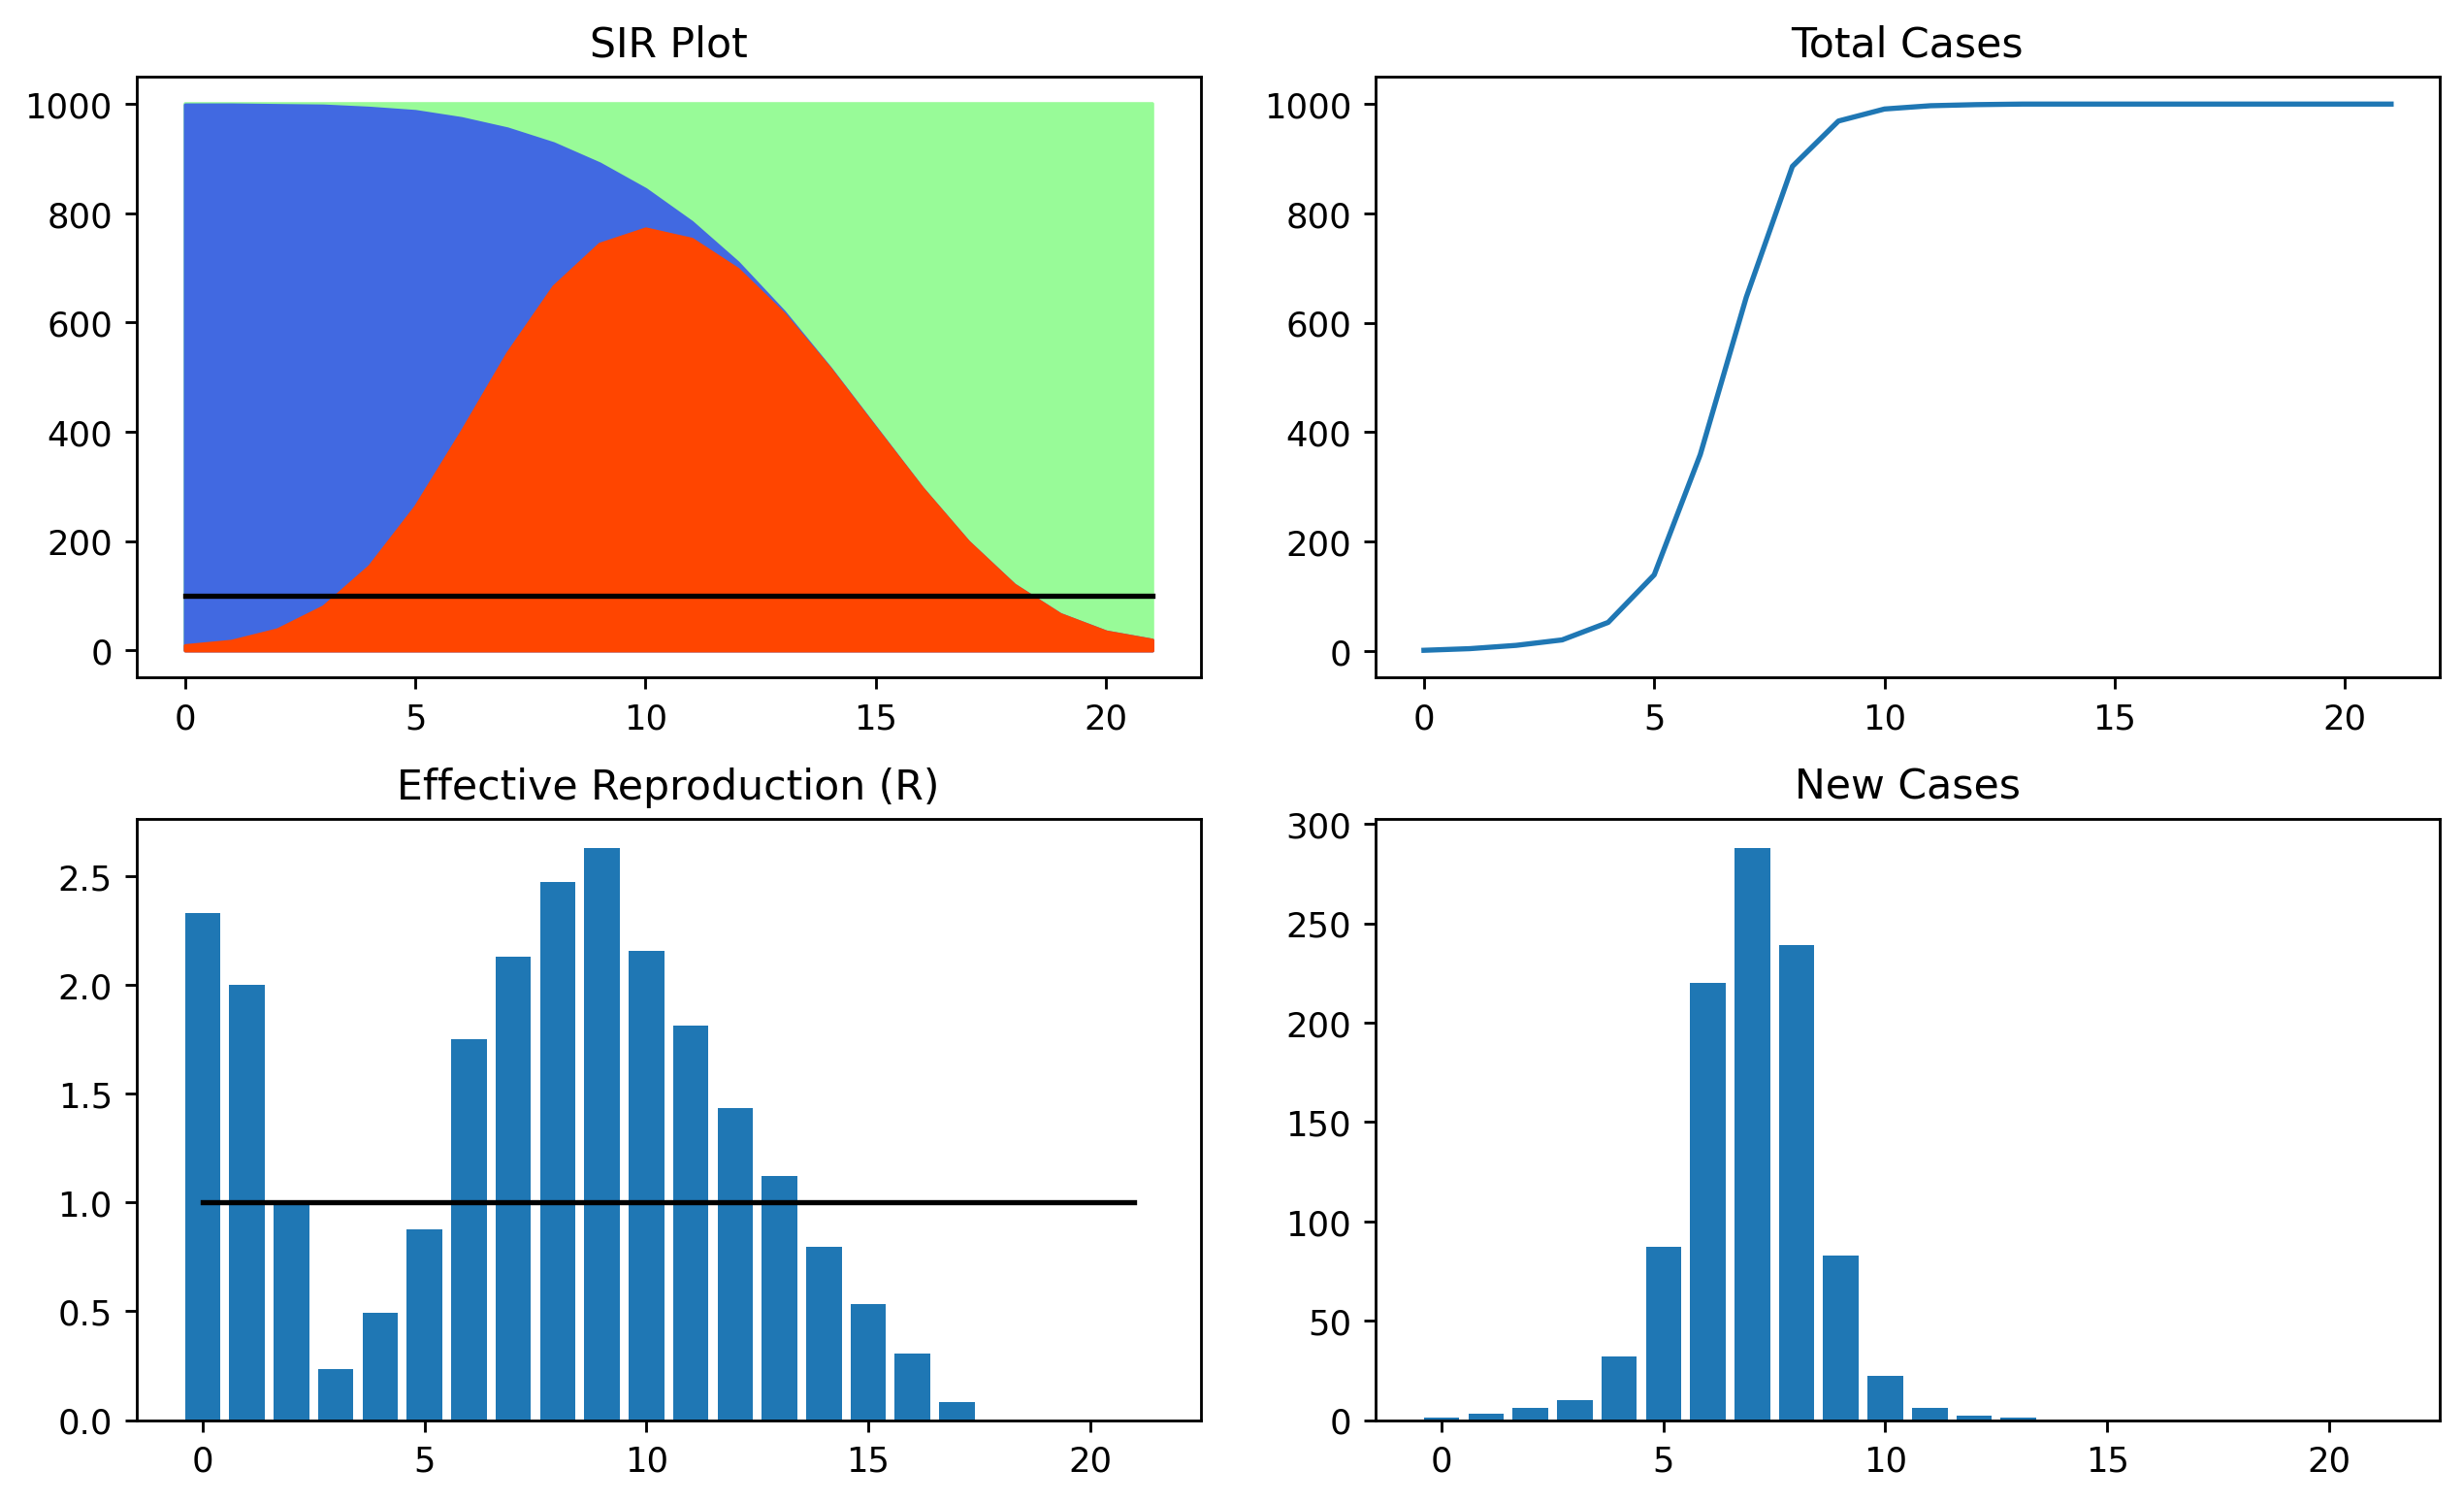
\includegraphics[width=6in, height=5.25in]{images/results/baseline.png}
        \caption{Baseline Statistics}
    \end{figure}
    
    \newpage
    \paragraph{} When we increase the ``connectedness" of the graph by increasing community centre count to 100 and average friend count to 20, the total duration falls down to 17 days, but the peak cases rise to 940. This was no surprise. We can say that the disease was encouraged to spread rapidly, and hence was over quickly. But of course, this is no solution to the problem
    \vspace{0.2in}
    \begin{figure}[h]
        \centering
        \includegraphics[width=6in, height=5.25in]{images/results/connectednessUp.png}
        \caption{Community Centres = 100, Average Friend Count = 20}
    \end{figure}
    
    \newpage
    \paragraph{} When we go to the opposite end and decrease the connectedness of the graph by having only 10 community centres and only 5 friends on average, we once again see the expected results. The peak cases comes down to 681, and total cases down to 977 (i.e. few people were unaffected). We still crossed the number of beds available though. The effective reproduction might seem counter intuitive at first peaking at almost 2.75, unlike the previous case where it didn't even reach 2.5. But on closer inspection, this is because the number of people causing secondary infections are lesser. What matters here is that during the rise in cases, it too was on an uptrend and was above 1, signalling the increase. When the cases peaked out, R started on a downtrend.
    \vspace{0.2in}
    \begin{figure}[h]
        \centering
        \includegraphics[width=6in, height=5.25in]{images/results/connectednessDown.png}
        \caption{Community Centres = 10, Average Friend Count = 5}
    \end{figure}
    
    \newpage
    \paragraph{} Next let us try changing the travel parameters, namely the travel probability and the travel strictness. With travel probability set to 0.9 and travel strictness at 0 i.e. no travel ban, we didn't see much difference from the baseline. The duration was the same and once again everyone was infected. In fact the peak cases slightly decreased, although this can be dismissed as noise. So why didn't the situation get drastically worse with everyone travelling? This was because in our model we had considered the population to be one giant cluster, without any smaller ``sub clusters". As a result there was no effect if people travelled or not. It's too late to go back and change the graph structure in code, but that's fine as we've got plenty of other parameters to work with. We also tried going the other extreme with a complete travel ban by setting the travel strictness to 1, and once again we didn't see any major difference.
    \begin{figure}[h]
        \centering
        \includegraphics[width=6in, height=5.25in]{images/results/highTravelProb.png}
        \caption{Average travel probability = 0.9}
    \end{figure}
    \newpage
    \begin{figure}[h]
        \centering
        \includegraphics[width=6in, height=5.25in]{images/results/noTravel.png}
        \caption{Travel ban strictness = 1}
    \end{figure}
    
    % Set1
    
    \newpage
    \paragraph{}
    Average friend count in this simulation is the degree of each node in the graph, which shows us how many nodes are connected to a single node.
    We have taken the base degree as 10 but as we increase this degree to 60 we see certain changes in our graphs.
    First the slope of the total cases graph increases which represent that the number of nodes infected increases at a faster rate. As can be seen through the new cases graph where we can see how fast all the population is infected.
    \vspace{0.2in}
    \begin{figure}[h]
        \centering
        \includegraphics[width=6in, height=5.25in]{images/set1/degree60.PNG}
        \caption{Average friend Count = 60}
    \end{figure}
    
    \newpage
    \paragraph{}
    Average Social distance is the measure in meters between 2 nodes. This is used to determine the physical distance between two nodes which is the sum of average social distance and social distance variation, this physical distance will be one of the parameter to decide whether an adjacent node can be infected or not since if this physical distance is larger than the infection radius the disease cannot be transmitted. From this we can easily concur that if we increase the average social distance between nodes, less nodes will be infected. As is visible in the graph, if we increase the average social distance to 2.2 from our base value of 1.25 we see in the SIR graph that the susceptible population is less than the base graph. Also the new cases graph is more spread out which means more time is taken for spreading of the infection.
    \vspace{0.2in}
    \begin{figure}[h]
        \centering
        \includegraphics[width=6in, height=5.25in]{images/set1/avgsocialdist2.2.PNG}
        \caption{Average Social Distance = 2.2}
    \end{figure}
    
    \newpage
    \paragraph{}
    To see whether contamination between two nodes is possible or not we have to see how many physical contacts a particular node makes. For this we have a parameter called as average physical contact between 2 nodes per day. For these physical contacts we check whether infection is possible between nodes considering other parameters also like immunity, quarantine probability etc. But if we keep other parameters we can say that if the average number of physical contacts increase the infection will spread faster, as is visible in the graph below where the average physical contact has been increased to 20 from base value.
    \vspace{0.2in}
    \begin{figure}[h]
        \centering
        \includegraphics[width=6in, height=5.25in]{images/set1/avgphysicalcontact20.PNG}
        \caption{Average number of physical contact between 2 people in a day = 20}
    \end{figure}
    
    \newpage
    \paragraph{}
    As depicted above that increasing the average physical contacts increase the infection rate in the population, but we know that many other factors are also working for determining the infection rate like if we increase the average physical contact to 20 as shown above but with that we increase the average immunity of the population also to 0.8 from base value of 0.2, we see that although more people are coming in contact but since the immunity is increased the chance getting infected gets decreased.
    In the graph below we can see the new cases graph is more spread out and in the SIR graph also the increase in susceptible cases is not sudden whereas it increases slowly.
    \vspace{0.2in}
    \begin{figure}[h]
        \centering
        \includegraphics[width=6in, height=5.25in]{images/set1/avgphysicalcontact20avgimmunity0.8.PNG}
        \caption{Average number of physical contact between 2 people in a day = 20 average immunity = 0.8}
    \end{figure}
    
    % Set2
    \newpage
    \paragraph{} For the baseline, we have kept quarantine strictness high which is quite likely in real scenario. But if we change it from 0.9 to 0.15, we observe that the disease takes more time to eradicate and also the peak number of cases is reached in less time.
    \vspace{0.2in}
    \begin{figure}[h!]
        \centering
        \includegraphics[width=6in, height=5.25in]{images/set2/strictness.PNG}
        \caption{Quarantine strictness = 0.15}
    \end{figure}
    
    \newpage
    \paragraph{} 
    Quarantine Probability - It represents the probability of an infected person to be quarantined.
    For reference we have taken quarantine probability to be 0.2.
    Changing it to 1, i.e if everyone being affected is quarantined, it is observed that number of peak cases is dropped and a few people are not affected at all. Although it is also observed that it takes more time for the disease to eradicate.
    \vspace{0.2in}
    \begin{figure}[h]
        \centering
        \includegraphics[width=6in, height=5.25in]{images/set2/probability1.PNG}
        \caption{Quarantine probability = 1}
    \end{figure}
    
    \vspace{0.2in}
    \newpage
    \paragraph{} On the other hand if quarantine probability is set to 0, it is observed that, the whole population is affected in less duration of time and peak number of cases is also increased.
    \vspace{0.2in}
    \begin{figure}[h]
        \centering
        \includegraphics[width=6in, height=5.25in]{images/set2/probability2.PNG}
        \caption{Quarantine probability = 0}
    \end{figure}
    
    \newpage
    \paragraph{} As reference we have taken number of available beds (hospital beds) sufficient for 10\% of the total population. If it is increased to 80\%, it is observed that disease doesn't affect the whole population, but there is no considerable changes in peak, daily new cases etc. This is due to the fact that we have increased the number of hospital beds but the probability of quarantining infected people is still low(0.2). If probability is increased to 0.8, it is observed that a drastic change occurs, the graphs flattens considerably, with less number of daily cases. The disease doesn't affect lot of people and the peak is decreases drastically.
    \vspace{0.2in}
    \begin{figure}[h]
        \centering
        \includegraphics[width=6in, height=5.25in]{images/set2/bed probability.PNG}
        \caption{Bed available = 800}
    \end{figure}
    
    \newpage
    \paragraph{} Next let's simulate a scenario where the vaccination drive is in full swing causing the immunity to go up, and naturally people are following a less stricter quarantining. No doubt, it is observed that peak cases drops with considerable number of people remaining unaffected, but the disease is prolonged. While it might not look great initially to have the disease prolonged, it also helps make sure most people get the beds they need leading to a lower mortality rate
    \vspace{0.2in}
    \begin{figure}[h]
        \centering
        \includegraphics[width=6in, height=5.25in]{images/set2/avgimmu.PNG}
        \caption{Average immunity = 0.8, Quarantine Strictness = 0.5}
    \end{figure}
    
    \vspace{0.2in}
    \newpage
    \paragraph{} For the reference we have taken the adherence to safety measures as 0 i.e. none. Now if we increase it to 0.4, i.e. simulating people wearing masks, sanitizing their hands etc. it is observed that the curve flattens a bit, peak reached is less, and total cases decreases.
    \vspace{0.2in}
    \begin{figure}[h]
        \centering
        \includegraphics[width=6in, height=5.25in]{images/set2/avgadh1.PNG}
        \caption{Average adherence to safety measures = 0.4}
    \end{figure}
    
    \vspace{0.2in}
    \newpage
    \paragraph{} Now if we further, increase adherence to 0.8 and decrease quarantine strictness to 0.6, the graph gets more flat and there is decrease in peak and total number of overall cases. This goes to show how important following safety measures is!
    \vspace{0.2in}
    \begin{figure}[h]
        \centering
        \includegraphics[width=6in, height=5.25in]{images/set2/avgadh2.PNG}
        \caption{Average adherence to safety measures = 0.8, Quarantine Strictness = 0.6}
    \end{figure}
    
    \newpage
    \paragraph{} In the next example we have set the parameters in such a way that a useful observation can be achieved, in case of widespread of the disease and during the peak of the pandemic, emergency field hospitals are set to increase the number of beds to accommodate the high number of active cases (beds available increased to 400, i.e 40\% of the population). As we are dealing at the peak of the pandemic, thus quarantine strictness and quarantine probability is also high(0.9).
    \vspace{0.2in}
    \begin{figure}[h]
        \centering
        \includegraphics[width=6in, height=5.25in]{images/set2/ex1.PNG}
        \caption{Beds available = 400, Quarantine Strictness = 0.9, Quarantine Probability = 0.9}
    \end{figure}
    \paragraph{} With these parameters, it is observed that increasing the number of beds available and high strictness and quarantining of people helps into slowing down the spread of the disease, and also it keeps the daily active cases much lower with drastic decrease in peak number of cases. 
    
    \newpage
    \paragraph{} Now in the coming example it is shown that if quarantine measures are not strictly followed even in case of high quarantine probability and more than enough number of beds available for the population the disease can be widespread and can affect the whole population, to depict this quarantine strictness is set to 0.1, probability to 8 and number of beds available to 800 for a 1000 population.
    Even though the beds are sufficient for whole population and nearly everyone getting affected is quarantined the disease affect the whole population and peak reached is high.
    \vspace{0.2in}
    \begin{figure}[h]
        \centering
        \includegraphics[width=6in, height=5.25in]{images/set2/ex2.PNG}
        \caption{Beds available = 800, Quarantine Strictness = 0.1, Quarantine Probability = 0.8}
    \end{figure}
    
    % Set3
    \vspace{0.2in}
    \newpage
    \paragraph{} Average duration of infection - It is the period(in days) that the infection affects the infected. We have taken the base degree for this variable as 9. But as we increase this degree to 25 we see certain changes in our graphs. The total epidemic duration increased to 38, but the peak cases remains nearly the same.
    \vspace{0.2in}
    \begin{figure}[h]
        \centering
        \includegraphics[width=6in, height=5.25in]{images/set3/1-Average duration.png}
        \caption{Average duration of infection = 25}
    \end{figure}
  
    \newpage
    \paragraph{}This probability is set on a daily basis. We have taken 0.05 as the reference value for this. When we increased it's value to 0.2 it is observed that the total cases falls down to 983 (i.e., 17 people were unaffected) and also a significant decrease in the reproduction rate. This is because the rate of spread will be low when the infected person dies. So the epidemic duration for this increases by 6 more days, as compared to the base graph.
    \vspace{0.2in}
    \begin{figure}[h]
        \centering
        \includegraphics[width=6in, height=5.25in]{images/set3/2-dying.png}
        \caption{Probability of infected person dying = 0.2}
    \end{figure}
    
    \newpage
    \paragraph{} Infection probability of the virus - The following is the probability that the virus infects i.e., spreads from one person to another given all favourable conditions. When we increased the value from 0.05 to 0.35, the total duration falls down to 16 days, but the peak raises to 945. Also the slope of the Total Cases graph increases which represents that the number of nodes infected increases at a faster rate. We can see from the graph that how fast all the population is infected.
    \vspace{0.2in}
    \begin{figure}[h]
        \centering
        \includegraphics[width=6in, height=5.25in]{images/set3/3-infection prob.png}
        \caption{Infection probability of the virus = 0.35}
    \end{figure}
    
    \newpage
    \paragraph{} Probability of infection to be asymptotic - This shows the probable range (0 to 1) of how asymptotic a infected person is. When we increased it's value from base value 0.1 to 0.6, we didn't see much difference from the baseline except that the Effective reproduction increased a bit at the beginning but decreased eventually. However the duration remained the same and everyone is affected.
    \vspace{0.2in}
    \begin{figure}[h]
        \centering
        \includegraphics[width=6in, height=5.25in]{images/set3/5-asymptotic.png}
        \caption{Probability of Infection to be asymptotic = 0.6}
    \end{figure}
    
    \newpage
    \paragraph{} Infection radius of the virus - This is the maximum physical distance(in metres) between two people after which the virus fails to spreads. When we changed the radius from 2 to 0.7, the graph gets a little flat and there is decrease in peak and in the total number of overall cases. As we can see in the graph the total cases are just 555 and the peak cases are around 200. Since the infection radius is less, the spreading rate is effectively low in this case. Because of this the duration also increased from 22 days to 68 days.
    \vspace{0.2in}
    \begin{figure}[h]
        \centering
        \includegraphics[width=6in, height=5.25in]{images/set3/4-radius.png}
        \caption{Infection radius of the virus = 0.7}
    \end{figure}

    \newpage
    \paragraph{} On the other hand when we did the reverse of the above condition i.e., slightly increase in the infection radius from 2 to 5, it is observed that the whole population is affected in less time and peak number of cases also got increased.
    \vspace{0.2in}
    \begin{figure}[h]
        \centering
        \includegraphics[width=6in, height=5.25in]{images/set3/6-radius.png}
        \caption{Infection radius of the virus = 5}
    \end{figure}
    
    \newpage
    \section{Conclusion}
        \paragraph{} Having analysed the simulation results and drawn necessary conclusions, let us now formally wrap everything up. The research started with identifying the problem statement and laying out the requirements. With that done, we then went through the literature available, to gain valuable insights to help us along the way. We also discovered that what we had planned to do, while wasn't unexplored territory, also wasn't done in the way we had planned to. Therefore we finalised the research plan, and began the simulation software development phase. Once that was nearing its end, we started with the testing and analysis phase, and followed it up with the final documentation phase.
        \paragraph{} This research which had started in the November of 2020, had spanned up to June of 2021. Of course, being busy with college work and jobs, we could find time only during the weekends to do this research. In spite of that, we think we have done a significant work, both in terms of the software development and simulation analysis.
        \paragraph{} In case one would like continue this research, he / she can find all the documentation including this one, as well as the Python code on GitHub at github.com/eeshaanachar/epidemic-simulation. As a starting point, we suggest remodelling the network structure to include clusters of population and to check the effect of travel parameters, as this was something we couldn't achieve owing to time constraints. From there one can think of newer parameters and / or outputs for the simulation. We also genuienly hope that the research would be carried out in pure interest and not because of another pandemic requiring this research.
	
	\newpage
	\section{References}
	    \subsection{Primary}
            \begin{itemize}
                \item Sanderson, G. (2020). Simulating an epidemic. Retrieved from \url{https://www.youtube.com/watch?v=gxAaO2rsdIs}
                
                \item Stevens, H. (2020). Why outbreaks like coronavirus spread exponentially, and how to “flatten the curve”. Retrieved from \url{https://www.washingtonpost.com/graphics/2020/world/corona-simulator}.
                
                \item Simler K. (2020). Outbreak. Retrieved from \url{https://meltingasphalt.com/interactive/outbreak}.
                
                \item Iyengar, S. (2019). Social Networks. Retrieved from \url{https://www.youtube.com/playlist?list=PLyqSpQzTE6M8CLBcLnq-f3vHRH-klC39L}
                
                \item Sanderson, G. (2020). Exponential growth and epidemics. Retrieved from \url{https://www.youtube.com/watch?v=Kas0tIxDvrg}
                
                \item Zaplotnik, Z., Gavrić, A., \& Medic L. (2020). Simulation of the COVID-19 pandemic on the social network of Slovenia. Retrieved from \url{https://journals.plos.org/plosone/article?id=10.1371/journal.pone.0238090}.
            \end{itemize}
            
        \subsection{Secondary}
            \begin{itemize}
                \item Cherry, J., Krogstad, P. (2004). SARS: The First Pandemic of the 21st Century. Retrieved from \url{https://doi.org/10.1203/01.PDR.0000129184.87042.FC}
                
                \item Ferguson, N., Cummings, D., Cauchemez, S. et al. (2005). Strategies for containing an emerging influenza pandemic in Southeast Asia. Retrieved from \url{https://doi.org/10.1038/nature04017}
                
                \item Jiang, S., Wang, K., Li, C. et al. (2017). Mathematical models for devising the optimal Ebola virus disease eradication.Retrieved from \url{https://doi.org/10.1186/s12967-017-1224-6}
                
                \item Zhao, P. (2020). A Social Network Model of the COVID-19 Pandemic. Retrieved from \url{https://doi.org/10.1101/2020.03.23.20041798}.
                
                \item Bansal, S., Grenfell, B. \& Meyers, L. (2007). When individual behaviour matters: homogeneous and network models in epidemiology. Retrieved from \url{https://doi.org/10.1098/rsif.2007.1100}
                
                \item Chao, D., Halloran, E. et al. (2010). FluTE, a Publicly Available Stochastic Influenza Epidemic Simulation Model. Retrieved from \url{https://doi.org/10.1371/journal.pcbi.1000656}
                
                \item Nguyen, D., Deguchi, H. et al. (2010). Agent-based simulation on avian influenza in Vietnam: Basic characteristics of the epidemic and efficiency evaluation of control measures. Retrieved from\\ \url{https://ieeexplore.ieee.org/abstract/document/5530215}
                
                \item Tuite, A., Eisenberg, M. et al. (2011). Cholera Epidemic in Haiti, 2010: Using a Transmission Model to Explain Spatial Spread of Disease and Identify Optimal Control Interventions. Retrieved from \url{www.researchgate.net/publication/50304455}
                
                \item Nassar, M., Meo, S. et al. (2018). Global seasonal occurrence of \\Middle East Respiratory Syndrome Coronavirus (MERS-CoV) infection. Retrieved from \url{www.researchgate.net/publication/326041885}
                
                \item Hossain, M. et al. (2020). The effects of border control and quarantine measures on the spread of COVID-19. Retrieved from \url{www.sciencedirect.com/science/article/pii/S1755436520300244}
            \end{itemize}
     
    \appendix
    
    \newpage
    \section{Research Team}
        \vspace{0.5in}
        \textbf{
            \hspace{0.6in} Eeshaan Achar
            \hspace{2in} Anuj Yadav
        }\\\\
        \includegraphics[scale=0.09]{images/Eeshaan.jpg}
        \hspace{0.5in}
        \includegraphics[scale=0.09]{images/set3/anuj.jpg}
        
        \vspace{0.5in}
        \textbf{
            \hspace{0.25in} Saurav Kumar
            \hspace{1.75in} Manjunath Badakar
        }\\\\
        \includegraphics[scale=0.2]{images/set2/Saurav photo.jpeg}
        \hspace{0.5in}
        \includegraphics[scale=0.302]{images/Manju_Badakar.jpg}
    
    \newpage
    \section{COs, POs and PSOs mapping for the Project work (CS84P)}
        \subsection{Course Outcomes}
        \begin{itemize}
        	\item[]\textbf{CO1:} Formulate the problem definition, conduct literature review and apply requirements analysis.
        	\item[]\textbf{CO2:} Develop and implement algorithms for solving the problem formulated.
        	\item[]\textbf{CO3:} Comprehend, present and defend the results of exhaustive testing and explain the major findings.
        \end{itemize}
    \subsection{Program Outcomes}
    	\begin{itemize}
    		\item[]\textbf{PO1:} Apply knowledge of computing, mathematics, science, and foundational engineering concepts to solve the computer engineering problems.
    		\item[]\textbf{PO2:} Identify, formulate and analyze complex engineering problems.
    		\item[]\textbf{PO3:} Plan, implement and evaluate a computer-based system to meet desired societal needs such as economic, environmental, political, healthcare and safety within realistic constraints.
    		\item[]\textbf{PO4:} Incorporate research methods to design and conduct experiments to investigate real-time problems, to analyze, interpret and provide feasible conclusion.
    		\item[]\textbf{PO5:} Propose innovative ideas and solutions using modern tools.
    		\item[]\textbf{PO6:} Apply computing knowledge to assess societal, health, safety, legal and cultural issues and the consequent responsibilities relevant to professional engineering practice.
    		\item[]\textbf{PO7:} Analyze the local and global impact of computing on individuals and organizations for sustainable development.
    		\item[]\textbf{PO8:} Adopt ethical principles and uphold the responsibilities and norms of computer engineering practice.
    		\item[]\textbf{PO9:} Work effectively as an individual and as a member or leader in diverse teams and in multidisciplinary domains.
    		\item[]\textbf{PO10:} Effectively communicate and comprehend.
    		\item[]\textbf{PO11:} Demonstrate and apply engineering knowledge and management principles to manage projects in multidisciplinary environments.
    		\item[]\textbf{PO12:} Recognize contemporary issues and adapt to technological changes for lifelong learning.
    	\end{itemize}
    \subsection{Program Specific Outcomes}
    	\begin{itemize}
    		\item[]\textbf{PSO1:} Problem Solving Skills: Ability to apply standard practices and mathematical
    		methodologies to solve computational tasks, model real world problems in the areas of
    		database systems, system software, web technologies and Networking solutions with an
    		appropriate knowledge of Data structures and Algorithms.
    		\item[]\textbf{PSO2:} Knowledge of Computer Systems: An understanding of the structure and work-
    		ing of the computer systems with performance study of various computing architectures.
    		\item[]\textbf{PSO3:} Successful Career and Entrepreneurship: The ability to get acquaintance with
    		the state of the art software technologies leading to entrepreneurship and higher studies.
    		\item[]\textbf{PSO4:} Computing and Research Ability : Ability to use knowledge in various domains
    		to identify research gaps and to provide solution to new ideas leading to innovations.
    	\end{itemize}
    \newpage
    \section{Publication Details}
    \paragraph{} We have consolidated the work done in this research into a research paper, and have submitted it to ``THE 28TH ASIA-PACIFIC SOFTWARE ENGINEERING CONFERENCE" (\url{https://apsec2021.seat.org.tw/}) that was originally planned to take place in Taipei, Taiwan, but now is being held virtually. This conference is an international conference and in their own words, ``The Asia-Pacific Software Engineering Conference (APSEC) has long been established as a premier regional conference that brings together researchers and practitioners from academia, industry and government to share the state of the art and the practice of software engineering, and to explore emerging challenges and solutions in software engineering innovation."
    \paragraph{} Unfortunately though, the conference dates are 6th to 9th of December, 2021. In spite of that, we decided to go with the said conference as it is an international one, is open to a wide variety of research work in the field of Computer Science and Software Engineering, and importantly is legit unlike most of the paid conferences that promise to get the paper published in a few hours / days. We believe that our work is worthy enough of getting the recognition, if any, through this conference.
    \vspace{0.25in}
    \begin{figure}[h!]
        \centering
        \includegraphics[scale=0.35]{images/submissionProof.png}
        \caption{Proof of Submission}
    \end{figure}
\end{document}